%% abtex2-modelo-trabalho-academico.tex, v-1.9.2 laurocesar
%% Copyright 2012-2014 by abnTeX2 group at http://abntex2.googlecode.com/ 
%%
%% This work may be distributed and/or modified under the
%% conditions of the LaTeX Project Public License, either version 1.3
%% of this license or (at your option) any later version.
%% The latest version of this license is in
%%   http://www.latex-project.org/lppl.txt
%% and version 1.3 or later is part of all distributions of LaTeX
%% version 2005/12/01 or later.
%%
%% This work has the LPPL maintenance status `maintained'.
%% 
%% The Current Maintainer of this work is the abnTeX2 team, led
%% by Lauro César Araujo. Further information are available on 
%% http://abntex2.googlecode.com/
%%
%% This work consists of the files abntex2-modelo-trabalho-academico.tex,
%% abntex2-modelo-include-comandos and abntex2-modelo-references.bib
%%

% ------------------------------------------------------------------------
% ------------------------------------------------------------------------
% abnTeX2: Modelo de Trabalho Academico (tese de doutorado, dissertacao de
% mestrado e trabalhos monograficos em geral) em conformidade com 
% ABNT NBR 14724:2011: Informacao e documentacao - Trabalhos academicos -
% Apresentacao
% ------------------------------------------------------------------------
% ------------------------------------------------------------------------

%-------------------------------------------------------------------------
% Modelo adaptado especificamente para o contexto do PPgSI-EACH-USP por 
% Marcelo Fantinato, com auxílio dos Professores Norton T. Roman, Helton
% H. Bíscaro, e Sarajane M. Peres, em 2015, com muitos agradecimentos aos 
% criadores da classe e do modelo base.
%-------------------------------------------------------------------------

\documentclass[
% -- opções da classe memoir --
12pt,				% tamanho da fonte
% openright,			% capítulos começam em pág ímpar (insere página vazia caso preciso)
oneside,			% para impressão apenas no anverso (apenas frente). Oposto a twoside
a4paper,			% tamanho do papel. 
% -- opções da classe abntex2 --
%chapter=TITLE,		% títulos de capítulos convertidos em letras maiúsculas
%section=TITLE,		% títulos de seções convertidos em letras maiúsculas
%subsection=TITLE,	% títulos de subseções convertidos em letras maiúsculas
%subsubsection=TITLE,% títulos de subsubseções convertidos em letras maiúsculas
% -- opções do pacote babel --
english,			% idioma adicional para hifenização
%french,				% idioma adicional para hifenização
%spanish,			% idioma adicional para hifenização
brazil				% o último idioma é o principal do documento
]{abntex2ppgsi}

% ---
% Pacotes básicos 
% ---
% \usepackage{lmodern}			% Usa a fonte Latin Modern			
% \usepackage[T1]{fontenc}		% Selecao de codigos de fonte.
\usepackage[utf8]{inputenc}		% Codificacao do documento (conversão automática dos acentos)
\usepackage{lastpage}			% Usado pela Ficha catalográfica
\usepackage{indentfirst}		% Indenta o primeiro parágrafo de cada seção.
\usepackage{color}				% Controle das cores
\usepackage{graphicx}			% Inclusão de gráficos
\usepackage{microtype} 			% para melhorias de justificação
\usepackage{pdfpages}     		%para incluir pdf
\usepackage{algorithm}			%para ilustrações do tipo algoritmo
\usepackage{mdwlist}			%para itens com espaço padrão da abnt
\usepackage[noend]{algpseudocode}			%para ilustrações do tipo algoritmo

% ---
% Pacotes adicionais, usados apenas no âmbito do Modelo Canônico do abnteX2
% ---
\usepackage{lipsum}				% para geração de dummy text
% ---

% ---
% Pacotes de citações
% ---
\usepackage[brazilian,hyperpageref]{backref}	 % Paginas com as citações na bibl
\usepackage[alf]{abntex2cite}	% Citações padrão ABNT

% ---
% Pacote para inserir comentários coloridos para autores trabalhar colaborativamente.
% ---
\usepackage[colorinlistoftodos, textwidth=20mm, textsize=footnotesize]{todonotes}
\newcommand{\victor}[1]{\todo[author=\textbf{Victor},color=green!30,caption={},inline]{#1}}
\newcommand{\karina}[1]{\todo[author=\textbf{Karina},color=red!30,caption={},inline]{#1}}

% --- 
% CONFIGURAÇÕES DE PACOTES
% --- 

% ---
% Configurações do pacote backref
% Usado sem a opção hyperpageref de backref
\renewcommand{\backrefpagesname}{Citado na(s) página(s):~}
% Texto padrão antes do número das páginas
\renewcommand{\backref}{}
% Define os textos da citação
\renewcommand*{\backrefalt}[4]{
	\ifcase #1 %
	Nenhuma citação no texto.%
	\or
	Citado na página #2.%
	\else
	Citado #1 vezes nas páginas #2.%
	\fi}%
% ---

% ---
% Informações de dados para CAPA e FOLHA DE ROSTO
% ---

%-------------------------------------------------------------------------
% Comentário adicional do PPgSI - Informações sobre o ``título'':
%
% Em maiúscula apenas a primeira letra da sentença (do título), exceto 
% nomes próprios, geográficos, institucionais ou Programas ou Projetos ou 
% siglas, os quais podem ter letras em maiúscula também.
%
% O subtítulo do trabalho é opcional.
% Sem ponto final.
%
% Atenção: o título da Dissertação na versão corrigida não pode mudar. 
% Ele deve ser idêntico ao da versão original.
%
%-------------------------------------------------------------------------
\titulo{Utilizando técnicas de Planejamento em IA para automatizar a geração de um Planejamento Instrucional de conteúdo adaptado a um ambiente e-learning}

%-------------------------------------------------------------------------
% Comentário adicional do PPgSI - Informações sobre o ``autor'':
%
% Todas as letras em maiúsculas.
% Nome completo.
% Sem ponto final.
%-------------------------------------------------------------------------
\autor{\uppercase{Victor Miranda Gonçalves Jatobá}}

%-------------------------------------------------------------------------
% Comentário adicional do PPgSI - Informações sobre o ``local'':
%
% Não incluir o ``estado''.
% Sem ponto final.
%-------------------------------------------------------------------------
\local{São Paulo}

%-------------------------------------------------------------------------
% Comentário adicional do PPgSI - Informações sobre a ``data'':
%
% Colocar o ano do depósito (ou seja, o ano da entrega) da respectiva 
% versão, seja ela a versão original (para a defesa) seja ela a versão 
% corrigida (depois da aprovação na defesa). 
%
% Atenção: Se a versão original for depositada no final do ano e a versão 
% corrigida for entregue no ano seguinte, o ano precisa ser atualizado no 
% caso da versão corrigida. 
% Cuidado, pois o ano da ``capa externa'' também precisa ser atualizado 
% nesse caso.
%
% Não incluir o dia, nem o mês.
% Sem ponto final.
%-------------------------------------------------------------------------
\data{2016}

%-------------------------------------------------------------------------
% Comentário adicional do PPgSI - Informações sobre o ``Orientador'':
%
% Se for uma professora, trocar por ``Profa. Dra.''
% Nome completo.
% Sem ponto final.
%-------------------------------------------------------------------------
\orientador{Profa. Dra. Karina Valdivia Delgado}

\tipotrabalho{Dissertação (Mestrado)}

\preambulo{
%-------------------------------------------------------------------------
% Comentário adicional do PPgSI - Informações sobre o texto ``Versão 
% original'':
%
% Não usar para Qualificação.
% Não usar para versão corrigida de Dissertação.
%
%-------------------------------------------------------------------------
Versão original
%-------------------------------------------------------------------------
% Comentário adicional do PPgSI - Informações sobre o ``texto principal do
% preambulo'':
%
% Para Qualificação, trocar por: Texto de Exame de Qualificação apresentado à Escola de Artes, Ciências e Humanidades da Universidade de São Paulo como parte dos requisitos para obtenção do título de Mestre em Ciências pelo Programa de Pós-graduação em Sistemas de Informação.
%
%-------------------------------------------------------------------------
\newline \newline \newline Dissertação apresentada à Escola de Artes, Ciências e Humanidades da Universidade de São Paulo para obtenção do título de Mestre em Ciências pelo Programa de Pós-graduação em Sistemas de Informação. 
%
\newline \newline Área de concentração: Metodologia e Técnicas da Computação
%-------------------------------------------------------------------------
% Comentário adicional do PPgSI - Informações sobre o texto da ``Versão 
% corrigida'':
%
% Não usar para Qualificação.
% Não usar para versão original de Dissertação.
% 
% Substituir ``xx de xxxxxxxxxxxxxxx de xxxx'' pela ``data da defesa''.
%
%-------------------------------------------------------------------------
\newline \newline \newline Versão corrigida contendo as alterações solicitadas pela comissão julgadora em xx de xxxxxxxxxxxxxxx de xxxx. A versão original encontra-se em acervo reservado na Biblioteca da EACH-USP e na Biblioteca Digital de Teses e Dissertações da USP (BDTD), de acordo com a Resolução CoPGr 6018, de 13 de outubro de 2011.}
% ---


% ---
% Configurações de aparência do PDF final

% alterando o aspecto da cor azul
\definecolor{blue}{RGB}{41,5,195}

% informações do PDF
\makeatletter
\hypersetup{
     	%pagebackref=true,
		pdftitle={\@title}, 
		pdfauthor={\@author},
    	pdfsubject={\imprimirpreambulo},
	    pdfcreator={LaTeX com abnTeX2 adaptado para o PPgSI-EACH-USP},
		pdfkeywords={abnt}{latex}{abntex}{abntex2}{qualificação de mestrado}{dissertação de mestrado}{ppgsi}, 
		colorlinks=true,       		% false: boxed links; true: colored links
    	linkcolor=blue,          	% color of internal links
    	citecolor=blue,        		% color of links to bibliography
    	filecolor=magenta,      		% color of file links
		urlcolor=blue,
		bookmarksdepth=4
}
\makeatother
% --- 

% --- 
% Espaçamentos entre linhas e parágrafos 
% --- 

% O tamanho do parágrafo é dado por:
\setlength{\parindent}{1.25cm}

% Controle do espaçamento entre um parágrafo e outro:
\setlength{\parskip}{0cm}  % tente também \onelineskip
\renewcommand{\baselinestretch}{1.5}

% ---
% compila o indice
% ---
\makeindex
% ---

	% Controlar linhas orfas e viuvas
  \clubpenalty10000
  \widowpenalty10000
  \displaywidowpenalty10000

% ----
% Início do documento
% ----
\begin{document}

% Retira espaço extra obsoleto entre as frases.
\frenchspacing 

% ----------------------------------------------------------
% ELEMENTOS PRÉ-TEXTUAIS
% ----------------------------------------------------------
% \pretextual

% ---
% Capa
% ---
%-------------------------------------------------------------------------
% Comentário adicional do PPgSI - Informações sobre a ``capa'':
%
% Esta é a ``capa'' principal/oficial do trabalho, a ser impressa apenas 
% para os casos de encadernação simples (ou seja, em ``espiral'' com 
% plástico na frente).
% 
% Não imprimir esta ``capa'' quando houver ``capa dura'' ou ``capa brochura'' 
% em que estas mesmas informações já estão presentes nela.
%
%-------------------------------------------------------------------------
\imprimircapa
% ---

% ---
% Folha de rosto
% (o * indica que haverá a ficha bibliográfica)
% ---
\imprimirfolhaderosto*
% ---

% ---
% inserir o sumario
% ---
\pdfbookmark[0]{\contentsname}{toc}
\tableofcontents*
\cleardoublepage
% ---



% ----------------------------------------------------------
% ELEMENTOS TEXTUAIS
% ----------------------------------------------------------
\textual



%-------------------------------------------------------------------------
% Comentário adicional do PPgSI - Informações sobre ``títulos de seções''
% 
% Para todos os títulos (seções, subseções, tabelas, ilustrações, etc):
%
% Em maiúscula apenas a primeira letra da sentença (do título), exceto 
% nomes próprios, geográficos, institucionais ou Programas ou Projetos ou
% siglas, os quais podem ter letras em maiúscula também.
%
%-------------------------------------------------------------------------
\chapter{Introdução}

Os Sistemas de Tutores Inteligentes (STI) são programas de software que dão suporte às atividades da aprendizagem \cite{gamboa2002} e atualmente são tão eficazes quanto o acompanhamento individualizado por um Tutor humano em sala de aula \cite{vanlehn2011}. Sendo o último, muito mais efetivo do que os métodos tradicionais de ensino, em que não há um acompanhamento personalizado \cite{bloom1984}. A arquitetura clássica de um STI levantada é composta por quatro componentes: modelo do Aluno; modelo do Especialista; modelo Instrucional ou Pedagógico e modelo da Interface \cite{kaplan1995}. Por definição todo STI deve ser adaptado e personalizado ao aprendizado de cada aluno \cite{woo1991} sendo o Planejamento Instrucional o processo que possibilita tal característica \cite{mohan2003}. Esse processo pode ser classificado em: planejamento de conteúdo, onde é selecionado o conteúdo para alcançar um determinado objetivo de aprendizagem \cite{vassileva1996} e planejamento de apresentação que constrói uma sequência ótima de interações entre o tutor e o aluno \cite{mohan2003}. Para que seja possível automatizar o processo de Planejamento Instrucional, técnicas de planejamento em Inteligência Artificial podem ser utilizadas \cite{cho2000, vassileva1996, brusilovsky2003}.

A plataforma virtual Make Your Time © possui ferramentas que ajudam estudantes que estão se preparando para exames e concursos públicos na etapa de planificação das atividades de estudos, gerando automaticamente uma planilha de horas de estudos, no acompanhamento do rendimento escolar por meio de gráficos de desempenho e na prática de recuperação do conteúdo com a disponibilização de questões. Porém, não existe nenhum mecanismo de inteligência que faça com que o sistema se adapte ao aprendizado do estudante ao longo do tempo, além de não fornecer, de forma cronológica, uma melhor sequência de estudos e questões para maximizar o aprendizado do estudante no prazo pré-determinado.

A proposta desse trabalho é aplicar as técnicas de planejamento em IA para automatizar a geração de um Planejamento Instrucional de conteúdo na plataforma Make Your Time.

\chapter{Objetivo}

O presente estudo propõe um planejador instrucional adaptativo que utiliza os níveis de aprendizado do aluno e os requisitos exigidos no edital do exame que este irá prestar. Para automatizar a criação do planejamento instrucional e garantir a adaptabilidade do sistema, um agente não humano fará uso de técnicas de planejamento apoiado em Inteligência Artificial e aprendizado de máquina.

Cita-se como objetivos específicos desse trabalho:
\begin{itemize}
	\item A definição de um modelo de estudante;
	\item Proposta e desenvolvimento de uma nova arquitetura para o ambiente EAD Make Your Time através das integrações do planejador proposto e do modelo do estudante;
\end{itemize}

\chapter{Metodologia}

\chapter{Fundamentos teóricos}

\section{Sistemas Tutores Inteligentes (STI)}

No final da década de 60 foram implementados uma série de sistemas sobre problemas em aritmética e recordação de vocabulário. Posteriormente outros sistemas surgiram com o intuito de fornecer exercícios e práticas em aritmética, selecionando problemas a partir do nível de dificuldade de cada estudante. Esses sistemas foram classificados como adaptativos e nomeados de Sistemas de Instrução Assistida por Computadores (CAI do inglês Computer-Assisted Instruction). Esse sistema é considerado o precursor dos Sistemas de Tutores Inteligentes \cite{sleeman1982}.

Os STIs são programas computacionais que utilizam técnicas de Inteligência Artificial, que de forma individualizada promovem o ensino e o aprendizado \cite{wenger1987}. Sendo assim, não se trata apenas de um sistema que examina resposta de usuários à questões \cite{sleeman1982}. \citeonline{vanlehn2011} demonstra que os STIs possuem uma maior eficiência para o aprendizado do que os métodos presentes em sistemas de tipos de tutoria mais tradicionais como os Computer Aided-Instruction (CAI), Computer-Based Instruction, Computer-Aided Learning, e o Computer-Based Training. Uma característica marcante dos STIs é que o acompanhamento à solução de um problema ou o aprendizado de um novo tópico acontece etapa por etapa, dando um feedback direto a partir da interação do usuário \cite{vanlehn2011}. Esses sistemas devem apresentar algumas características. Primeiro, o conteúdo do tema ou especialidade deve ser codificada de tal forma que o sistema computacional possa ser capaz de acessar as informações, fazer inferências ou resolver problemas. Segundo, o sistema deve ser capaz de deduzir um valor de aproximação do aprendizado do aluno. Por fim, a parte de tutoria deve implementar estratégias para reduzir a diferença entre o conhecimento do especialista e o conhecimento do estudante \cite{polson2013}. Além disso, o sistema deve monitorar a execução do plano, e replanejar quando necessário devendo ser adaptável ao aprendizado do aluno \cite{woo1991}.

A arquitetura clássica dos STIs (\ref{fig:figura1}) é composta por basicamente quatro componentes \cite{kaplan1995}:

\begin{enumerate}
	\item \textbf{Modelo do Aluno}: nesse módulo são tratadas as características individuais do aluno.
	\item \textbf{Modelo do Especialista}: detém o conhecimento sobre as disciplinas e assuntos no formato de regras de produção, estereótipos, etc.
	\item \textbf{Modelo Instrucional ou pedagógico}: aqui está a parte da personalização do conteúdo para o estudante. Contém o conhecimento sobre as estratégias e práticas para seleciona-las em função das características dos alunos.
	\item \textbf{Modelo da Interface}: intermedia a iteração entre o tutor e o aluno. São divididos em três tipos: o aluno, o professor e o programador do sistema.
\end{enumerate}

%-------------------------------------------------------------------------
% Figura 1
%
% Fonte própria
%-------------------------------------------------------------------------
\begin{figure}[H]% H manda colocar exatamente nessa posição no texto (relativa aos parágrafos anterior e posterior)
	\centering
	\caption{Arquitetura clássica de um STI}
	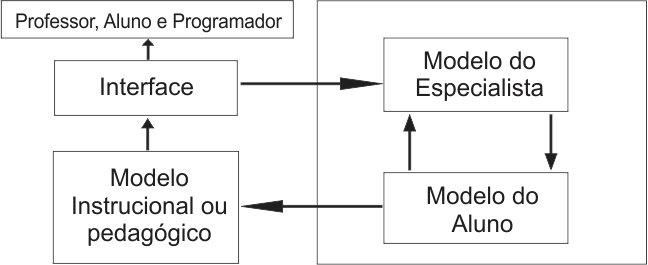
\includegraphics{figura1.png}
	\label{fig:figura1}
	\source{Kaplan e Rock, 1995}
\end{figure}

\section{Planejamento instrucional}

É de fundamental importância que em sistemas inteligentes e adaptáveis de educação a distância via WEB forneçam automaticamente, de forma personalizada, o conteúdo a ser aprendido pelo aluno \cite{brusilovsky2003}. Conteúdo, nesse trabalho, corresponde a questões. O propósito é motivar o estudante e ter certeza de que ele é capaz de resolver os problemas da base de domínio. No entanto não é de interesse fazer com que seja gasto muito tempo tentando resolver todos os problemas ou resolver problemas parecidos repetidas vezes. O grande dilema é que a seleção dos problemas deve ser desafiador sem ser frustrante. Assim o planejamento das questões deve manter os estudantes interessados em continuar os estudos até o final \cite{cho2000}. Para a geração automática da sequência das questões é possível utilizar a técnica de Planejamento Instrucional.

O planejamento instrucional é o processo que possibilita a organização do conteúdo de forma consistente, coerente e continuada de um processo instrucional definido de acordo com as características de cada aluno e com os objetos educacionais utilizados \cite{vassileva1996, mohan2003}. Foi inicialmente proposto por \cite{peachey1986} e posteriormente adotados em muitos STIs. É através do planejamento instrucional que os sistemas tutores promovem o aprendizado individualizado \cite{mohan2003}, identificando e selecionando as estratégias para suprir as deficiências no conhecimento de cada aluno \cite{polson2013}.

O planejemanto instrucional pode ser dividido em dois tipos: planejamento de conteúdo que seleciona o conteúdo para alcançar um determinado objetivo de aprendizagem \cite{vassileva1996} e planejamento de apresentação que constrói uma sequência ótima de interações entre o tutor e o aluno \cite{mohan2003}. Esse processo pode ser automatizado através do uso de técnicas de planejamento em Inteligência Artificial \cite{cho2000, vassileva1996, brusilovsky2003, garrido2008}.

\section{Planejamento em IA e Planejamento instrucional}

Técnicas de Planejamento em IA permitem a criação de rotas de aprendizagem baseado nas preferências dos estudantes. São geradas automaticamente uma sequência de ações (planos) que satisfazem um dado objetivo (propriedade do mundo), por exemplo, a geração de uma sequência de leituras, lições, escritas, etc., que o estudante precisa seguir para completar o curso \cite{castillo2010}. Com o uso dessa técnica em STIs, se obtem um plano de ações que definem o sequenciamento de recursos adaptado para o estudante \cite{challco2012}.
Um dos primeiros trabalhos que usa técnicas de planejemento em IA dentro de plataformas e-learning foi \cite{peachey1986}. Posteriormente \citeonline{vassileva1998} criou um sistema na WWW que gera dinamicamente um curso instrucional baseado em representações explícitas da estrutura dos conceitos / tópicos que foi mantido separado das matérias de ensino. \citeonline{ullrich2008} foi um dos pioneiros a utilizar planejamento hierárquico de rede de tarefas (HTN-planning, Hierarchical Task Network Planning) para gerar planejamento instrucional. O sistema foi nomeado de PAIGOS e na implementação foi utilizado o planejador jSHOP2 \cite{nau2003}. Em \citeonline{challco2014} foram criadas estratégias para a geração de planos instrucionais baseado em Aprendizado Colaborativo e foi proposto o jSHOP2ip, uma versão do jSHOP2 específico para planejamento instrucional para esse tipo de ambiente.

\section{A plataforma WEB}

O Make Your Time © é uma plataforma virtual que ajuda estudantes que estão se preparando para algum exame ou concurso público na etapa de planificação das atividades de estudos onde, utilizando técnicas de Inteligência Artificial, traça o perfil (baseado nas dificuldades, disponibilidade e facilidade de aprendizado) do estudante e gera, automaticamente, uma planilha de estudos contendo as disciplinas e a carga horária a ser dedicada ao estudo em cada período do dia em um calendário semanal. Ele sugere ao usuário, por exemplo, quais disciplinas ele deve estudar na sexta-feira pela manhã e quantas horas deve dedicar a cada uma naquele período. Também provê ferramentas que podem ajudar no acompanhamento do rendimento escolar, como gráficos de desempenho, sinalização dos conteúdos que ele possui maior dificuldade, tempo restante para o exame, e o seu desempenho em relação aos outros usuários na plataforma. Por fim é disponibilizado questões de concursos e exames anteriores para o aluno poder testar o conhecimento.
Falar sobre a técnica utilizada no algoritmo que gera a planilha de estudos.
Até o dado momento a ferramenta não disponibiliza nenhum tipo de conteúdo preparatório e não possui nenhum mecanismo inteligente para se adaptar ao aprendizado do estudante ao longo do tempo. O sistema gera uma planilha de estudos que não é reajustada às atuais dificuldades e necessidades que se apresentam ao longo do processo de aprendizagem do estudante. Também não existe uma forma cronológica e inteligente de geração de atividades e tarefas que faça com que o aluno atinja seus objetivos e maximize o seu aprendizado até a data do exame que ele irá prestar.
A plataforma foi financiada por recursos próprios, possuindo atualmente cerca de 200 usuários com uma taxa de 15\% de usuários ativos. O seu acesso está disponível no endereço eletrônico: www.makeyourtime.com.br. 

\chapter{Cronograma}


% ----------------------------------------------------------
% ELEMENTOS PÓS-TEXTUAIS
% ----------------------------------------------------------
\postextual
% ----------------------------------------------------------

% ----------------------------------------------------------
% Referências bibliográficas
% ----------------------------------------------------------
\bibliography{victorjatoba-referencias}


%---------------------------------------------------------------------
% INDICE REMISSIVO
%---------------------------------------------------------------------
%%%%%MF\phantompart
%%%%%MF\printindex
%---------------------------------------------------------------------

\end{document}
